\section{جهت ۱: هندسهٔ ترتیبی مستقیم}
\label{sec:d1}
\begin{keybox}[شاخه: \branch{direction1-ordinal-geometry}]
پنج \lr{grade vector} مستقیماً در فضای مشترک تصویر و متن آموخته می‌شوند و ترتیب، با سه \lr{constraint} هندسی \lr{ladder}، \lr{path} و \lr{anchor}، روی خود همین بردارها اعمال می‌شود. \lr{text encoder} فقط یک بار برای \lr{initialisation} به کار می‌رود.
\end{keybox}

شکل~\ref{fig:wf-d1} گردش کار کامل جهت ۱ را نشان می‌دهد. داده و تقسیم آن همان مدل پایه است و تفاوت در \lr{block}های مدل (الف) و \lr{loss function} (ب) است؛ \lr{protocol} آزمایش‌ها در شکل~\ref{fig:proto-d1} آمده است.

\begin{landscape}
\begin{figure}[p]
\centering
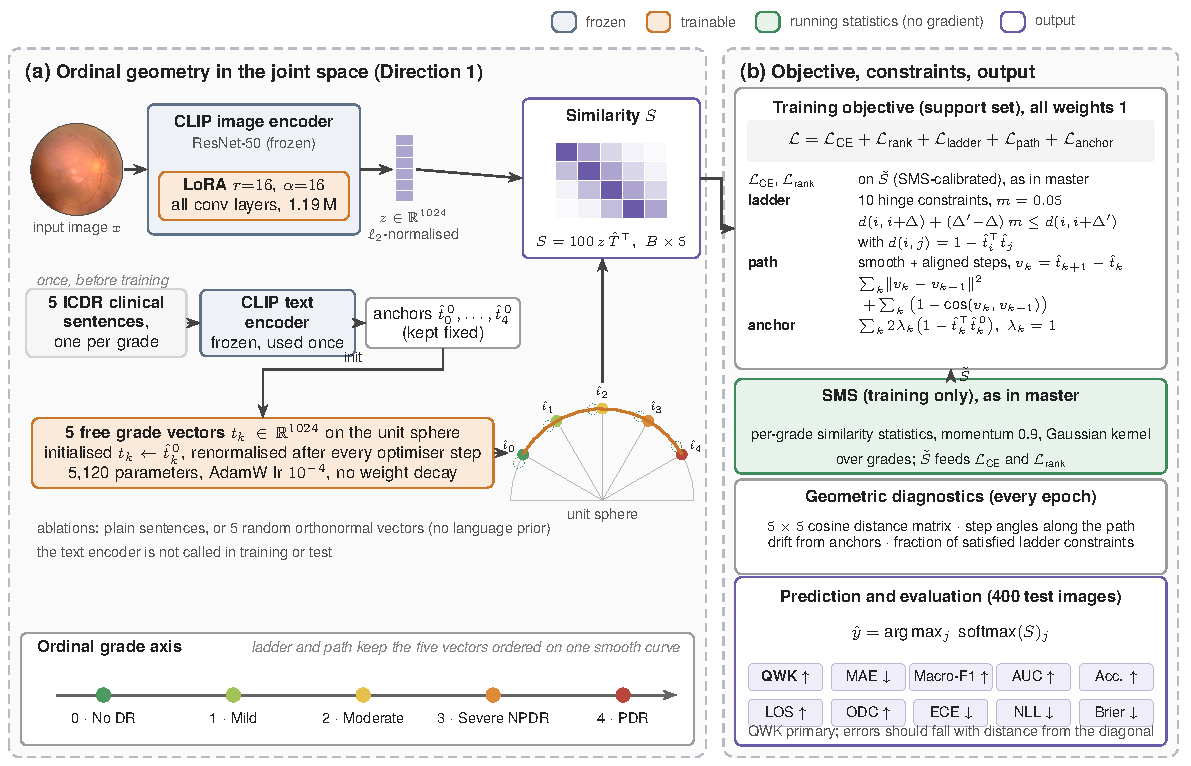
\includegraphics[width=\linewidth]{workflow_d1}
\caption{گردش کار کامل جهت ۱: بردارهای آزاد درجه که یک بار از جمله‌های بالینی مقداردهی می‌شوند، \lr{constraint}های \lr{ladder}، \lr{path} و \lr{anchor} روی همان بردارها و \lr{geometric diagnostics} هر \lr{epoch}.}
\label{fig:wf-d1}
\end{figure}
\end{landscape}

% ------------------------------------------------------------------
\subsection{انگیزه و شکاف پژوهشی}
در مدل پایه، ترتیب از راه توکن‌های ورودی \lr{text encoder} وارد می‌شود. \lr{rank token}ها شاید به هم نزدیک باشند، اما \lr{text encoder} یک تابع غیرخطی و \lr{frozen} است و هیچ تضمینی نیست که \lr{prototype}ها خروجی، یعنی همان بردارهایی که \lr{similarity} با آن‌ها سنجیده می‌شود، ترتیب را حفظ کنند. از سوی دیگر روش‌های جدید \lr{few-shot} مانند \lr{CLAP} \cite{clap} \lr{prototype}ها را مستقیماً در فضای مشترک می‌آموزند و با یک \lr{anchor} به متن اولیه نزدیک نگه می‌دارند؛ اما این روش‌ها هیچ رابطه‌ای میان کلاس‌ها در نظر نمی‌گیرند. جهت ۱ این دو را ترکیب می‌کند: پنج \lr{grade vector} مستقیماً در فضای مشترک آموخته می‌شوند و ترتیب، با \lr{geometric constraints}، روی خود همین بردارها اعمال می‌شود.

\begin{figure}[H]
\begin{diagram}
  \node[frozen=3.6cm] (a) {\textbf{Master model}\\ order injected into text encoder input};
  \node[box=3.6cm,below=of a] (a2) {Frozen nonlinear encoder may break ordering};
  \node[frozen=3.6cm,left=14mm of a] (b) {\textbf{CLAP}\\ free prototype + anchor};
  \node[box=3.6cm,below=of b] (b2) {No inter-class relationship is modelled};
  \node[train=6cm,below=12mm of $(a2)!0.5!(b2)$] (c) {\textbf{Dir.~1:} free grade vector + geometric ordinal constraints on those vectors};
  \draw[arr] (a)--(a2); \draw[arr] (b)--(b2); \draw[arr] (a2)--(c); \draw[arr] (b2)--(c);
\end{diagram}
\caption{شکاف پژوهشی جهت ۱: ترکیب \lr{prototype} آزاد (مانند \lr{CLAP}) با \lr{constraint} ترتیبی مستقیم.}
\label{fig:d1-gap}
\end{figure}

% ------------------------------------------------------------------
\subsection{تفاوت با مدل پایه}
\begin{table}[H]
\caption{آنچه در جهت ۱ تغییر می‌کند و آنچه ثابت می‌ماند}
\label{tab:d1-diff}
\centering\small
\begin{tabularx}{\textwidth}{@{}p{3.6cm} X X@{}}
\toprule
\textbf{جزء} & \textbf{مدل پایه} & \textbf{جهت ۱}\\
\midrule
نمایش درجه‌ها & \lr{prompt} \lr{learnable} از \lr{text encoder} \lr{frozen} & پنج بردار آزاد ۱۰۲۴-بعدی روی \lr{unit sphere}\\
\lr{text encoder} در آموزش & در هر گام فراخوانی می‌شود & فقط یک بار برای \lr{initialisation}\\
\lr{constraint} ترتیبی روی نمایش & \lr{interpolation} توکن‌ها & \lr{distance ladder}، \lr{smooth path}، \lr{anchor} به متن\\
\lr{image branch}، داده، \lr{SMS}، \lr{loss} رتبه، \lr{metric}ها، آموزش & \multicolumn{2}{l}{یکسان (بخش‌های \ref{sec:data} تا \ref{sec:metrics})}\\
\bottomrule
\end{tabularx}
\end{table}

% ------------------------------------------------------------------
\subsection{معماری}
\begin{figure}[H]
\begin{diagram}
  \node[datan=3.2cm] (s) {5 ICDR clinical sentences};
  \node[frozen=3.2cm,right=8mm of s] (te) {CLIP text encoder (frozen)};
  \node[datan=3.2cm,right=8mm of te] (t0) {$t^0_0\dots t^0_4$: anchors};
  \node[train=3.6cm,below=12mm of t0] (t) {$t_0\dots t_4$: free parameters\\ normalise after each step};
  \node[datan=2.6cm,left=46mm of t] (x) {Image};
  \node[train=3cm,below=of x] (v) {CLIP RN50 + LoRA};
  \node[box=3.6cm,below=of t] (g) {Geometric constraints:\\ ladder · path · anchor};
  \node[box=3.4cm,below=16mm of $(v)!0.5!(t)$] (sim) {$s = 100\cdot z\,\hat{t}^{\top}$};
  \node[box=3cm,below=of sim] (sms) {SMS (train only)};
  \node[lossn=3.4cm,below=of sms] (l1) {CE + rank-aware loss};
  \node[lossn=3.4cm,right=10mm of l1] (lg) {Geometric losses};
  \node[lossn=6cm,below=of $(l1)!0.5!(lg)$] (lt) {Total loss, Eq.~\ref{eq:d1-loss}};
  \draw[arr] (s)--(te); \draw[arr] (te)--(t0); \draw[arr] (t0)--node[elabel,right]{init}(t);
  \draw[arr] (x)--(v); \draw[arr] (v) |- (sim); \draw[arr] (t) -- (sim);
  \draw[arr] (sim)--(sms); \draw[arr] (sms)--(l1);
  \draw[arr] (t)--(g); \draw[darr] (t0.east) -- ++(5mm,0) |- (g.east);
  \draw[arr] (g) -- (lg); \draw[arr] (l1)--(lt); \draw[arr] (lg)--(lt);
  \begin{scope}[on background layer]\node[group,fit=(s)(te)(t0)] (gi) {};\end{scope}
  \node[grouplabel,anchor=south] at (gi.north) {Once, before training};
\end{diagram}
\archlegend
\caption{معماری جهت ۱. \lr{text encoder} فقط در \lr{initialisation} به کار می‌رود و در آموزش و آزمون حذف می‌شود.}
\label{fig:d1-arch}
\end{figure}

% ------------------------------------------------------------------
\subsection{\lr{initialisation} \lr{grade vector}ها}
هر \lr{grade vector} با کدگذاری یک جملهٔ بالینی مطابق مقیاس \lr{ICDR} \cite{icdr} توسط \lr{text encoder} \lr{frozen} آغاز می‌شود و نسخهٔ نرمال‌شدهٔ همین بردار به‌عنوان \lr{anchor} $\hat{t}^{0}_k$ نگه داشته می‌شود. در \lr{ablation}ها دو مقداردهی دیگر هم بررسی می‌شود: جمله‌های ساده (برای نمونه \lr{``A fundus photograph with mild non-proliferative diabetic retinopathy.''}) و پنج بردار متعامد تصادفی بدون هیچ دانش زبانی.

\begin{table}[H]
\caption{جمله‌های بالینی \lr{initialisation} (به زبان اصلی، همان‌گونه که به \lr{encoder} داده می‌شوند)}
\label{tab:d1-sent}
\centering\small
\begin{tabularx}{\textwidth}{@{}c X@{}}
\toprule
\textbf{درجه} & \textbf{جمله}\\
\midrule
۰ & \ensent{A fundus photograph showing no diabetic retinopathy, with normal retinal vasculature and no microaneurysms or hemorrhages.}\\
۱ & \ensent{A fundus photograph showing mild non-proliferative diabetic retinopathy, characterized by the presence of microaneurysms only.}\\
۲ & \ensent{A fundus photograph showing moderate non-proliferative diabetic retinopathy, with multiple microaneurysms, dot and blot hemorrhages, hard exudates, or cotton wool spots, less than severe.}\\
۳ & \ensent{A fundus photograph showing severe non-proliferative diabetic retinopathy, with extensive intraretinal hemorrhages in four quadrants, venous beading, or intraretinal microvascular abnormalities.}\\
۴ & \ensent{A fundus photograph showing proliferative diabetic retinopathy, characterized by neovascularization on the optic disc or elsewhere, vitreous hemorrhage, or preretinal hemorrhage.}\\
\bottomrule
\end{tabularx}
\end{table}

\begin{figure}[H]
\begin{diagram}
  \node[decision] (q) at (0,0) {Init type};
  \node[train=3.4cm] (a) at (-4.2,-2.0) {ICDR clinical sentences\\ (main model)};
  \node[box=3.4cm] (b) at (0,-2.0) {Plain sentences\\ (ablation)};
  \node[box=3.4cm] (c) at (4.2,-2.0) {5 random orthonormal\\ vectors (ablation)};
  \node[frozen=7.6cm] (e) at (-2.1,-3.75) {Frozen CLIP text encoder, then $\ell_2$-normalise};
  \node[datan=11.8cm] (o) at (0,-5.3) {$t_k \leftarrow \hat{t}^{\,0}_k$ \quad and keep $\hat{t}^{\,0}_k$ fixed as the anchor};
  \draw[arr] (q.west) -| (a.north);
  \draw[arr] (q.south) -- (b.north);
  \draw[arr] (q.east) -| (c.north);
  \draw[arr] (a.south) -- (a.south |- e.north);
  \draw[arr] (b.south) -- (b.south |- e.north);
  \draw[arr] (e.south) -- (e.south |- o.north);
  \draw[arr] (c.south) -- (c.south |- o.north);
  \node[elabel,right=1mm] at ($(c.south)!0.5!(c.south |- o.north)$) {no text encoder};
\end{diagram}
\caption{سه گزینهٔ مقداردهی \lr{grade vector}ها.}
\label{fig:d1-init}
\end{figure}

% ------------------------------------------------------------------
\subsection{\lr{ordinal geometric constraints}}
همهٔ \lr{constraint}ها روی بردارهای نرمال‌شدهٔ $\hat{t}_k$ و با \lr{cosine distance} $d(i, j) = 1 - \hat{t}_i^{\top} \hat{t}_j$ تعریف می‌شوند.

\subsubsection{\lr{distance ladder}}
از دید هر درجه، درجهٔ نزدیک‌تر باید از درجهٔ دورتر نزدیک‌تر باشد و این تفاوت با فاصلهٔ درجه‌ها \lr{margin}‌ای متناسب داشته باشد. برای پنج درجه، ۱۰ \lr{constraint} از این نوع وجود دارد:
\begin{equation}
\mathcal{L}_{\mathrm{ladder}} = \sum_{i} \sum_{1 \le \Delta < \Delta' \le K-1-i} \max\!\Big(0,\ d(i, i{+}\Delta) - d(i, i{+}\Delta') + (\Delta' - \Delta)\, m\Big), \qquad m = 0.05
\label{eq:ladder}
\end{equation}

\subsubsection{\lr{smooth path}}
پنج بردار باید روی یک خم یک‌بعدی و هموار روی \lr{sphere} قرار بگیرند تا ترتیب درجه‌ها در هندسه دیده شود. با گام‌های $v_k = \hat{t}_{k+1} - \hat{t}_k$، دو جزء تعریف می‌شود: هموار بودن (مشتق دوم کوچک) و هم‌جهت بودن گام‌های پیاپی:
\begin{equation}
\begin{gathered}
\mathcal{L}_{\mathrm{smooth}} = \sum_{k=1}^{K-2} \lVert v_k - v_{k-1} \rVert^2, \qquad \mathcal{L}_{\mathrm{align}} = \sum_{k=1}^{K-2} \big(1 - \cos(v_k, v_{k-1})\big),\\
\mathcal{L}_{\mathrm{path}} = \mathcal{L}_{\mathrm{smooth}} + \mathcal{L}_{\mathrm{align}}
\end{gathered}
\label{eq:path}
\end{equation}

\subsubsection{\lr{anchor}}
در \lr{regime} \lr{1-shot} یا \lr{2-shot}، بردارهای آزاد به‌آسانی \lr{overfitting} می‌کنند و دانش زبانی اولیه را از دست می‌دهند. \lr{anchor} هر بردار را به نقطهٔ آغازش نزدیک نگه می‌دارد. روی \lr{unit sphere}، مجذور \lr{Euclidean distance} برابر $2(1 - \cos)$ است:
\begin{equation}
\mathcal{L}_{\mathrm{anchor}} = \sum_k \lambda_k \lVert \hat{t}_k - \hat{t}^{0}_k \rVert^2 = \sum_k 2 \lambda_k \big(1 - \hat{t}_k^{\top} \hat{t}^{0}_k\big)
\label{eq:anchor}
\end{equation}
در مدل اصلی همهٔ $\lambda_k$ برابر ۱ هستند. دو وزن‌دهی دیگر در \lr{ablation} بررسی می‌شوند: وزن متناسب با معکوس ریشهٔ فراوانی هر درجه در دادهٔ آموزش (با میانگین ۱)، و وزن \lr{CLAP} که برابر میانگین احتمال \lr{zero-shot} درجهٔ درست روی تصاویر \lr{support} همان درجه است.

\begin{figure}[H]
\centering
\begin{latin}
\begin{tikzpicture}[x=1cm,y=1cm]
  % sphere arc with five grade vectors
  \draw[rulegray,thick] (0,0) circle (3.2);
  \fill[navy] (0,0) circle (1.5pt);
  \foreach \a/\k/\n in {150/0/0,125/1/1,100/2/2,75/3/3,50/4/4} {
    \draw[->,navy!70] (0,0) -- (\a:3.2);
    \fill[accent] (\a:3.2) circle (2.4pt);
    \node[font=\footnotesize] at (\a:3.65) {$\hat t_{\k}$};
  }
  \draw[accent,very thick] (150:3.2) arc (150:50:3.2);
  \foreach \a in {154,129,104,79,54} \draw[densely dotted,green!40!black] (\a:2.55) circle (0.12);
  \draw[<->,thick,green!40!black] (150:2.1) arc (150:125:2.1);
  \draw[<->,thick,green!40!black] (150:1.4) arc (150:100:1.4);
  \node[box=4.6cm,anchor=west] at (4.2,2.2) {\textbf{Ladder:} $d(0,1)<d(0,2)<d(0,3)<d(0,4)$ with margin $m$};
  \node[box=4.6cm,anchor=west] at (4.2,0.4) {\textbf{Path:} consecutive steps aligned \& equal-length (red arc)};
  \node[box=4.6cm,anchor=west] at (4.2,-1.4) {\textbf{Anchor:} each $\hat t_k$ stays near $\hat t^0_k$ (dotted circles)};
\end{tikzpicture}
\end{latin}
\caption{سه \lr{constraint} هندسی روی \lr{grade vector}ها. \lr{ladder} ترتیب فاصله‌ها، مسیر شکل کلی و \lr{anchor} پیوند با دانش زبانی را حفظ می‌کند.}
\label{fig:d1-geom}
\end{figure}

% ------------------------------------------------------------------
\subsection{\lr{loss function} کل}
\begin{equation}
\mathcal{L} = \mathcal{L}_{\mathrm{CE}}(\tilde{s}, y) + \mathcal{L}_{\mathrm{rank}}(\tilde{s}, y) + \mathcal{L}_{\mathrm{ladder}} + \mathcal{L}_{\mathrm{path}} + \mathcal{L}_{\mathrm{anchor}}
\label{eq:d1-loss}
\end{equation}
همهٔ وزن‌ها برابر ۱ هستند و $\tilde{s}$ همان \lr{similarity} \lr{calibrated} با \lr{SMS} است (رابطهٔ~\ref{eq:sms}). \lr{distance-weighted pairwise loss} (رابطهٔ~\ref{eq:pair}) در مدل اصلی جهت ۱ وجود ندارد و فقط در \lr{ablation} «+ \lr{pairwise loss}» افزوده می‌شود.

\begin{table}[H]
\caption{اجزای \lr{loss function} جهت ۱}
\label{tab:d1-loss}
\centering\small
\begin{tabularx}{\textwidth}{@{}p{3cm} p{2.6cm} c X@{}}
\toprule
\textbf{جزء} & \textbf{روی چه چیزی} & \textbf{وزن} & \textbf{نقش}\\
\midrule
\lr{cross-entropy} & $\tilde{s}$ & ۱ & طبقه‌بندی درست\\
\lr{ranking-aware loss} & $\tilde{s}$ & ۱ & شکل \lr{unimodal} \lr{similarity} هر تصویر\\
\lr{ladder} (\ref{eq:ladder}) & $\hat t_k$ & ۱ & ترتیب فاصله‌ها میان درجه‌ها\\
مسیر (\ref{eq:path}) & $\hat t_k$ & ۱ & قرار گرفتن درجه‌ها روی یک خم هموار\\
\lr{anchor} (\ref{eq:anchor}) & $\hat t_k,\hat t^0_k$ & ۱ & جلوگیری از \lr{overfitting} و حفظ دانش زبانی\\
\bottomrule
\end{tabularx}
\end{table}

% ------------------------------------------------------------------
\subsection{بهینه‌سازی}
\lr{grade vector}ها با \lr{AdamW} و همان \lr{learning rate} $10^{-4}$ اما بدون \lr{weight decay} آموخته می‌شوند، چون \lr{weight decay} روی \lr{parameter}ی که دوباره به \lr{sphere} تصویر می‌شود فقط اندازهٔ گام مؤثر را تغییر می‌دهد. پس از هر گام \lr{optimizer}، هر بردار دوباره به طول واحد نرمال می‌شود. بقیهٔ تنظیمات همان جدول~\ref{tab:train} است. \lr{parameter}های \lr{trainable} \LRE{۱٬۱۸۸٬۲۷۲} (\lr{LoRA}) به‌اضافهٔ $5\times1024$ = \LRE{۵٬۱۲۰} (\lr{grade vector}ها)، در مجموع \LRE{۱٬۱۹۳٬۳۹۲} هستند.

\begin{figure}[H]
\begin{diagram}
  \node[box=3cm] (f) {Compute total loss};
  \node[box=3cm,right=of f] (b) {Backpropagation};
  \node[train=3.2cm,right=of b] (o) {AdamW step\\ LoRA: weight decay $10^{-4}$\\ $t$: no weight decay};
  \node[train=3cm,below=of o] (n) {$t_k \leftarrow t_k/\lVert t_k\rVert$};
  \node[box=3cm,left=of n] (d) {End of epoch: log geometric diagnostics};
  \draw[arr] (f)--(b); \draw[arr] (b)--(o); \draw[arr] (o)--(n); \draw[arr] (n)--(d); \draw[darr] (d) -| (f);
\end{diagram}
\caption{یک گام بهینه‌سازی در جهت ۱. \lr{normalisation} پس از هر گام بردارها را روی \lr{sphere} نگه می‌دارد.}
\label{fig:d1-opt}
\end{figure}

% ------------------------------------------------------------------
\subsection{داده، ارزیابی و \lr{geometric diagnostics}}
داده، \lr{protocol} \lr{few-shot}، \lr{preprocessing} و همهٔ \lr{metric}های بخش~\ref{sec:metrics} بدون تغییر به کار می‌روند: ۲۴ اجرا برای مدل اصلی ($k \in \{-1, 0, 1, 2, 4, 8, 16, 32\}$ با ۳ \lr{seed})، آزمون روی ۴۰۰ تصویر و \lr{QWK} به‌عنوان \lr{metric} اصلی. در حالت \lr{zero-shot}، مدل همان \lr{classifier} \lr{zero-shot} \lr{CLIP} با جمله‌های بالینی است. افزون بر \lr{metric}ها، در پایان هر \lr{epoch} چهار تشخیص هندسی ذخیره می‌شود:
\begin{enumerate}[label=\arabic*.]
\item ماتریس \lr{cosine distance} $5\times5$ بین درجه‌ها؛
\item زاویهٔ چرخش میان گام‌های پیاپی \lr{path}؛
\item فاصلهٔ هر بردار از \lr{anchor}‌اش؛
\item سهم \lr{constraint}های \lr{ladder} برقرار (از ۱۰ \lr{constraint}).
\end{enumerate}

% ------------------------------------------------------------------
\subsection{\lr{baseline}ها و \lr{ablation}ها}
مقایسه شامل مدل \lr{master}، همهٔ مدل‌های جدول~\ref{tab:baselines} و دو نسخه از \lr{CLAP} است. \lr{CLAP} \lr{matched} با جمله‌های ساده آغاز می‌شود، وزن \lr{anchor} \lr{CLAP} را به کار می‌برد، فقط \lr{loss} \lr{CE} و \lr{anchor} دارد و \lr{LoRA} تصویر را حفظ می‌کند. \lr{CLAP} \lr{official} یک \lr{linear probe} روی ویژگی‌های \lr{frozen} است: بدون \lr{LoRA}، با \lr{SGD} و نرخ \LRE{۰٫۱} به مدت ۳۰۰ \lr{epoch} و بدون \lr{early stopping}.

\begin{table}[H]
\caption{\lr{ablation}ها جهت ۱}
\label{tab:d1-abl}
\centering\small
\begin{tabularx}{\textwidth}{@{}p{4.6cm} X@{}}
\toprule
\textbf{آزمایش} & \textbf{تغییر نسبت به مدل اصلی}\\
\midrule
بدون \lr{ladder} / بدون \lr{path} / بدون \lr{anchor} & وزن همان \lr{constraint} صفر\\
بدون \lr{geometric constraints} & هر سه \lr{constraint} صفر\\
فقط \lr{CE} و هندسه & بدون \lr{loss} رتبه و \lr{SMS}\\
مقداردهی با جمله‌های ساده & جمله‌های کوتاه به‌جای جمله‌های بالینی\\
مقداردهی متعامد تصادفی & بدون هیچ دانش زبانی\\
\lr{anchor} با معکوس ریشهٔ فراوانی & $\lambda_k \propto 1/\sqrt{N_k}$\\
+ \lr{pairwise loss} & افزودن \lr{distance-weighted pairwise loss}\\
\bottomrule
\end{tabularx}
\end{table}

\begin{figure}[H]
\centering
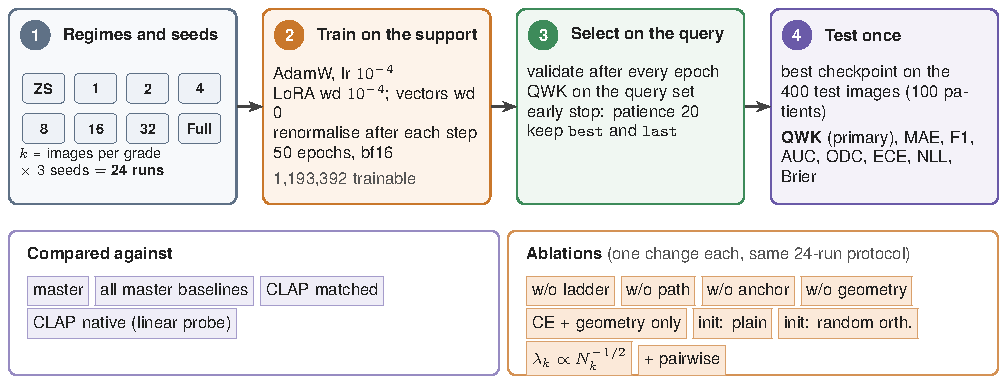
\includegraphics[width=\linewidth]{protocol_d1}
\caption{\lr{protocol} آزمایش‌های جهت ۱.}
\label{fig:proto-d1}
\end{figure}

\begin{figure}[H]
\begin{diagram}
  \node[train=4.4cm] (a) {Phase 1: Dir.~1 · 24 runs};
  \node[box=4.4cm,below=of a] (b) {Compare with master, Dir.~2 \& Dir.~3 from shared cache};
  \node[decision,below=of b] (c) {Dir.~1 is best?};
  \node[train=4.2cm,below=12mm of c,xshift=30mm] (d) {Phase 2: 9 baselines + 10 ablations};
  \node[box=4.2cm,below=12mm of c,xshift=-30mm] (e) {Tables from existing runs only};
  \node[lossn=4.2cm,below=of d] (f) {Geometric diagnostics for $k=8$};
  \draw[arr] (a)--(b); \draw[arr] (b)--(c);
  \draw[arr] (c) -| node[elabel,above,pos=0.3]{yes} (d); \draw[arr] (c) -| node[elabel,above,pos=0.3]{no} (e); \draw[arr] (d)--(f);
\end{diagram}
\caption{گردش کار آزمایش‌های جهت ۱.}
\label{fig:d1-flow}
\end{figure}
